\documentclass[11pt]{article}

\usepackage[letterpaper,top=2cm,bottom=2cm,left=2cm,right=2cm,marginparwidth=1.75cm]{geometry}
\usepackage{hyperref}
\usepackage{biblatex}
\addbibresource{Bib.bib}
\usepackage{mathtools}
\DeclarePairedDelimiterXPP\BigOSI[2]%
  {\mathcal{O}}{(}{)}{}%
  {\SI{#1}{#2}}
\usepackage{xcolor}
\usepackage{empheq}
\usepackage[most]{tcolorbox}
\usepackage{amsmath}
\usepackage{amssymb}
\usepackage{mathrsfs}
\usepackage[utf8]{inputenc}
\usepackage{graphicx}
\usepackage{float}
\usepackage{parskip}
\usepackage{comment}
\usepackage{mhchem}
 \usepackage{tabularx}
 \usepackage{titling}
 \usepackage{amsmath,environ}
 \usepackage[explicit]{titlesec}
\usepackage{fancyhdr}
\usepackage{braket}
\setlength{\droptitle}{3em} 

\title{Statistical Thermodynamics}
\author{Thomas Brosnan}
\date{Notes taken in Professor Graham Cross' class, Hilary Term 2024}


\newtcbox{\mymath}[1][]{%
    nobeforeafter, math upper, tcbox raise base,
    enhanced, colframe=blue!30!black,
    colback=blue!30, boxrule=1pt,
    #1}
\tcbset{highlight math style={boxsep=2mm,,colback=blue!0!green!0!red!0!}}

\newenvironment{bux}{\empheq[box=\tcbhighmath]{align}}{\endempheq}
\newenvironment{bux*}{\empheq[box=\tcbhighmath]{align*}}{\endempheq}
\renewenvironment{flalign}{\empheq[box=\tcbhighmath]{align}}{\endempheq}
\newcommand{\hsp}{\hspace{8pt}}

\newcommand*{\sectionFont}{%
  \LARGE\bfseries
}

    
\numberwithin{equation}{section}

\makeatletter
\let\Title\@title % Copy the title to a new command
\makeatother

%change this RGB value to change the section background colour 
\definecolor{mycolor1}{RGB}{255, 117, 26}
\colorlet{SectionColour}{mycolor1}
%subsection background colour 
\definecolor{mycolor2}{gray}{0.8}
\colorlet{subSectionColour}{mycolor2}
%subsubsection background colour 
\definecolor{mycolor3}{RGB}{255,255,255}
\colorlet{subsubSectionColour}{mycolor3}


\begin{document}

\maketitle

\newpage
\topskip0pt
\vspace*{\fill}
\begin{center}
\Large
    " Put a cool quote here or your lame "
    
    -Thomas Brosnan
\end{center}
\vspace*{\fill}
\newpage 
\tableofcontents
% For \section
 \titleformat{\section}[block]{\sectionFont}{}{0pt}{%
 \fcolorbox{black}{SectionColour}{\noindent\begin{minipage}{\dimexpr\textwidth-2\fboxsep-2\fboxrule\relax}\thesection  \hsp #1 {\strut} \end{minipage}}}
% For \subsection
 \titleformat{\subsection}[block]{\bfseries}{}{0pt}{%
 \fcolorbox{black}{subSectionColour}{\noindent\begin{minipage}{\dimexpr\textwidth-2\fboxsep-2\fboxrule\relax}\thesubsection  \hsp #1 {\strut} \end{minipage}}}
% For \section*
 \titleformat{name=\section, numberless}[block]{\sectionFont}{}{0pt}{%
 \fcolorbox{black}{SectionColour}{\noindent\begin{minipage}{\dimexpr\textwidth-2\fboxsep-2\fboxrule\relax} #1 {\strut} \end{minipage}}}
  % For \subsection*
 \titleformat{name=\subsection, numberless}[block]{\bfseries}{}{0pt}{%
 \fcolorbox{black}{subSectionColour}{\noindent\begin{minipage}{\dimexpr\textwidth-2\fboxsep-2\fboxrule\relax} #1 {\strut} \end{minipage}}}
 % For \subsubsection
 \titleformat{\subsubsection}[block]{\bfseries}{}{0pt}{%
 \fcolorbox{black}{subsubSectionColour}{\noindent\begin{minipage}{15cm}\thesubsubsection \hsp #1 {\strut} \end{minipage}}}
  % For \subsubsection*
 \titleformat{name=\subsubsection, numberless}[block]{\bfseries}{}{0pt}{%
 \fcolorbox{black}{subsubSectionColour}{\noindent\begin{minipage}{15cm} #1 {\strut} \end{minipage}}}
\newpage 
%header 
\pagestyle{fancy}
\fancyhf{} % Clear all header and footer fields
\fancyhead[L]{\Title}
\fancyhead[R]{\nouppercase{\leftmark}}
\fancyfoot[C]{-~\thepage~-}
\renewcommand{\headrulewidth}{1pt}











%starting document 
\normalsize
\newpage
\section{Concepts and Terminology }
\subsection{System macrostate}
\begin{itemize}
    \item Properties at large scale of the system when we know constraining thermodynamic parameters such as $P$,$V$ and $T$. 

\end{itemize}
\subsection{Quantum microstate }
\begin{itemize}
    \item Each quantum state is a separate and distinct microstate of the system.  
\end{itemize}

\subsection{Weakly coupled systems }
\begin{itemize}
    \item We assume weakly coupled systems. These are isolated systems such that the total macro-parameters $E,V,N$, are constant. Weak coupling implies that the energy levels of a single particle are effectively unchanged by particle interactions, but the interaction is sufficiently large to allow energy exchange. This means that at equilibrium the system must have a common temperature. 

This assumption makes the quantum mechanics involved easier, as coupled systems in quantum mechanics can be quite complex where as simple systems like a gas of $H_2$ can be solved analytically (eigenvalues of vibration,rotation and translation). 
\end{itemize}

\subsection{Locality} 
\begin{itemize}
    \item Localised particles are particles that are restricted to a certain place like a lattice for example. This way each particle of the lattice is \textit{distinguishable}, i.e. it can be told apart from the other particles in the gas due to its position. If particles in a system are non-localised they are \emph{indistinguishable}. 
\end{itemize}

\subsection{Bosons and Fermions}
\begin{itemize}
    \item In the case of indistinguishable particles we have two cases. Consider a two state system with two single particle states (orbitals) $a$ and $b$ and a wave function $\Psi$ describing the system.  We assume (weakly coupled systems ) that the particles are non-interacting so that we can write the wavefunction as a product of the two states: 
\begin{bux}
    \begin{split}
        \Psi(1,2) = \psi_a(1)\psi_b(2) ~~~ or ~~~ \Psi(2,1) = \psi_a(1)\psi_b(2)
    \end{split}
\end{bux}
Where here there are two possibilities for the states as the particles are indistinguishable. Quantum mechanics tells us that the wavefunction must be a linear combination of all the (equally likely thus same amplitude) possible states , so we write: 
\begin{bux}
    \begin{split}
\label{eqn:1.1}
        \Psi(1,2) \propto  \psi_a(1)\psi_b(2) \pm  \psi_a(1)\psi_b(2)
    \end{split}
\end{bux}
The $\pm$ here indicates the two possibilities with respect to particle exchange. If we swap two particles and the system is symmetric (i.e. we get a $+$) then these particles are \emph{Bosons}. And we can have any number of them in a single state, as if the states $a=b$ \ref{eqn:1.1} is not 0. 

However if we swap two particles and the system is anti-symmetric (now we get a $-$ sign) then the particles are \emph{Fermions} and we can only have one fermion per state, as \ref{eqn:1.1} is $0$ if $a=b$.  This is the Pauli exclusion principle. 

\end{itemize}

\subsection{Probability of microstates}
\begin{itemize}
    \item The probability of finding the system in a microstate $l$ is given by the number of times the system was found in that microstate $n(l)$ divided by the total number of states $\sum_ln(l)=r$: 
\begin{bux}
    \begin{split}
        P(l) = \frac{n(l)}{r}
    \end{split}
\end{bux}
Note that this means $\sum_lP(l)  =1$. This probability allows us to calculate average values of quantities. The average value of a quantity $\braket{A}$, is given by: 
\begin{bux}
    \begin{split}
      \braket{A}   = \sum_lA(l)P(l) = \frac{1}{r}\sum_lA(l)n(l) 
    \end{split}
\end{bux}

\item To realize this property, observations must be on a time scale that is long in comparison with the time for
the system to randomize (come to equilibrium), known as the \emph{relaxation time}.  
\end{itemize}

\subsection{Ensemble average}
\begin{itemize}
    \item An ensemble average or thermal average is the average over a large number of replicas of the entire system. A replica realizes one microstate of the system and it is the collection of replicas we call an ensemble.  

The ensemble can also be used to determine $P(l)$, and is postulated to be equivalent to the time sampling of a single system. This is essentially assuming the system is constantly jumping from state to state, essentially randomly. This assumption that these two averages, over time and over all possible states is known as the \emph{ergodic hypothesis}. 
\end{itemize}


\subsection{Fundamental assumption of statistical thermodynamics}
\begin{itemize}
    \item A system in thermal equilibrium is equally likely to be in any of the microstates accessible to it. 
\end{itemize}
\begin{itemize}
    \item This is the assumption of equal \textit{a priori probabilities}. 
\end{itemize}

\newpage
\section{Entropy and Temperature}
\subsection{Physics Principle }
\begin{itemize}
    \item Using the postulate we had earlier of a priori probabilities, we can say that since the system is equally likely to be any state then and assuming our system moves randomly from one microstate to the next, then it it is far more likely for the system, when not in equilibrium to evolve towards a state with higher number of microstates $\Omega$ as there are just more of them The system has more ways of arriving at those scenarios then the ones with smaller $\Omega$.  

Another way of seeing that the most probable macrostate is indeed the one realised by the maximum number of microstates is because this is where the system spends most its time, as it is far more likely to jump to a state with large $\Omega$. This is what we meant 
by the ergodic hypothesis. This essentially coincides with the definition of equilibrium, the system spends most it’s  time where there are a lot of states.  

In the next section Cross uses a specific spin system example to introduce entropy but we don't need to do that we can keep it more general as Manuela did in the Statistical Physics I modal. The following few sections are taken from my note from that class. 
\end{itemize}

\subsection{Combined system}
\begin{itemize}
    \item Consider an isolated system split, by a partition into two subsystems, 1 and 2 (with out loss of generality we can say that the system 1 is larger than 2). The systems have there own thermodynamic variables $E_1,V_1,N_1$ and $E_2,V_2,N_2$, respectively. The system is in equilibrium. At some point we allow energy exchange between the to systems. The two systems can now be considered one, described by the quantities $E,V$ and $N$, where $E= E_1+E_2$.  The number of microstates for this system is now: 
\begin{bux}
    \begin{split}
\label{eqn:2.1}
        \Omega(E_1,E_2,V,N)  = \Omega_1(E_1,V_1,N_1)\Omega_2(E_2,V_2,N_2)
    \end{split}
\end{bux}
This is because fundamentally $\Omega$ tells us how many different configurations of the system there are that result in the same energy, but system 1 and 2 are independent so naturally, the amount of different configurations is the product of the number of configurations of each subsystem.  
\end{itemize}

\subsubsection{Entropy}
\begin{itemize}
    \item Now we return to our two systems that have just been allowed to exchange energy. We want to know how $E_1$ and consequently $E_2 = E-E_1$, change as the system moves to a new equilibrium position. We know that we have to maximise the number of microstates $\Omega = \Omega_1\Omega_2$, so if $E_1^{\ast}$ and $E_2^{\ast} = E - E_1^{\ast}$ are the values of the energy's at equilibrium. Then taking the derivative of $\Omega = \Omega_1\Omega_2$ with respect to $E_1$, we must have that: 
\begin{bux}
    \begin{split}
       \Omega_2 \frac{\partial \Omega_1}{\partial E_1}\bigg\rvert_{E_1=E_1^{\ast}} +   \Omega_1\frac{\partial E_2}{\partial E_1} \frac{\partial \Omega_2}{\partial E_2}\bigg\rvert_{E_2=E_2^{\ast}} = 0
    \end{split}
\end{bux}
Now $\frac{\partial E_2}{\partial E_1}=-1$ as  $E_2 = E-E_1$, so we can divide this equation by $\Omega_1\Omega_2$ to get: 
\begin{bux}
    \begin{split}   
\label{eqn:4.34}
& \frac{1}{\Omega_1} \frac{\partial \Omega_1}{\partial E_1}\bigg\rvert_{E_1=E_1^{\ast}} -   \frac{1}{\Omega_2}\frac{\partial \Omega_2}{\partial E_2}\bigg\rvert_{E_2=E_2^{\ast}} = 0 \\ 
& \implies \frac{\partial \ln(\Omega_1)}{\partial E_1}\bigg\rvert_{E_1=E_1^{\ast}} = \frac{\partial \ln(\Omega_2)}{\partial E_2}\bigg\rvert_{E_2=E_2^{\ast}}
    \end{split}
\end{bux}
\item We can now introduce the quantity $\beta =  \frac{\partial \ln(\Omega)}{\partial E}\bigg\rvert_{E=E_1^{\ast}+E_2^{\ast}}$, So that the above equation \ref{eqn:4.34} can be written as $\beta_1 = \beta_2$.  We know that in thermodynamics equilibrium between two systems is reached when their temperatures are the same $T_1 = T_2$.  Naively we might say $\beta \propto T$ , but if we remember that temperature is defined as $T \equiv \frac{\partial E}{\partial S}$, then looking at the definition of $\beta$, it makes much more sense to write $\beta \propto \frac{1}{T}$ as now at equilibrium: 
\begin{bux}
    \begin{split}
         \frac{\partial S}{\partial E} =  \frac{1}{T} \propto \beta =  \frac{\partial \ln(\Omega)}{\partial E}
    \end{split}
\end{bux}
From the left most and right most expressions we can get an expression for entropy! If we denote the constant of proportionality between $\beta$ and $T$ as $1/k$, i.e. $\beta = \frac{1}{kT}$, Then entropy can be written as: 
\begin{bux}
    \begin{split}
\label{eqn:2.5}
        S = k \ln(\Omega)
    \end{split}
\end{bux}
This expression makes sense as if adding two systems together results in the number of microstates being the product of the original two systems $\Omega$'s, then the natural way to turn this into entropy would be a function that separates products into sums, as entropy of two systems add together, its an extensive variable. The most suitable function for this task is naturally the logarithm.  The constant of proportionality here $k$, is Boltzmann's constant.  

\item We can repeat this experiment, now allowing particles to be exchanged so that $N$ may vary too.  This means that we have a similar extra expression: 
\begin{bux}
    \begin{split}
  \frac{\partial \ln(\Omega_1)}{\partial N_1}\bigg\rvert_{N_1=N_1^{\ast}} = \frac{\partial \ln(\Omega_2)}{\partial N_2}\bigg\rvert_{N_2=N_2^{\ast}} 
    \end{split}
\end{bux}
Again we know from thermodynamics that the system is at equilibrium when the values $(T,\mu)$ are the same for both subsystems. So we must have that the following two equations are equivalent: 
\begin{bux}
    \begin{split}
          & d(\ln(\Omega))  =  \frac{\partial \ln(\Omega)}{\partial E } dE +  \frac{\partial \ln(\Omega)}{\partial N } dN  \\ 
 &\iff  \frac{dS}{k} = \frac{1}{kT}dE - \frac{\mu}{kT}dN
    \end{split}
\end{bux}
Which is true if we have $S = k\ln(\Omega)$.  If we have a system that is only changing particles, Since we can write $dS = 1/TdE-PdV+\mu dN$, if $V$ and $E$ are constant such that $dE=dV=0$, then we have that 
\begin{bux}
    \begin{split}
        \mu = - T \left( \frac{\partial S}{\partial N}\right)_{V,E}
    \end{split}
\end{bux}
This happens in chemical reactions.  

\end{itemize}
\newpage
\section{Partition functions }
\subsection{Probabilities }
\begin{itemize}
    \item We consider two systems in both \textit{thermal} and \textit{diffusive} (particle exchange) contact, one system is a reservoir and the other is far smaller in scale. We consider members of an ensemble comprising identical replicas of the system + reservoir, one copy for each quantum state of the combination. The system plus reservoir have total number of particles $N_0$ and internal energy $E_0$.  

The probability of the system being in a single microstate $i$ with particle number $N_i$ and energy $E_i$ is proportional to the number of microstates $\Omega(E,N)$. Since we have fixed the system in a single microstate $i$ $\Omega_{\rm system}(E_i,N_i) =1 $, the number of microstates of the reservoir is $\Omega_{\rm reservoir}(E_0-E_i,N_0-N_i)$. The number of microstates of the total volume is the product of the number of microstates of these two smaller systems, as we saw in \ref{eqn:2.1}. So we can write the probability of the system having a microstate with $E_i,N_i$ as: 
\begin{bux}
    \begin{split}
        P(E_i,N_i) \propto \Omega_{\rm system}(E_i,N_i)\Omega_{\rm reservoir}(E_0-E_i,N_0-N_i) = \Omega_{\rm reservoir}(E_0-E_i,N_0-N_i)
    \end{split}
\end{bux}
Then using $\Omega= e^{S/k}$ as per \ref{eqn:2.5}, we can write the relative probability (we will worry about the pre-factors later) of two states with $E_i,N_i$ and $E_j,N_j$ respectively as: 
\begin{bux}
    \begin{split}
        \frac{P(E_i,N_i)}{P(E_j,N_j)} = e^{\frac{S_i-S_j}{k}}
    \end{split}
\end{bux}
We can then perform a taylor expansion around $N=N_0$ and $E=E_0$ as $\frac{E_i}{E_0}, \frac{N_i}{N_0} << 1$ as the system is much smaller then the reservoir. of these entropys as they are of the form $S_i(E_0-E_i,N_0-N_i)$: 
\begin{bux}
    \begin{split}
        S_i(E_0-E_i,N_0-N_i) \approx S(E_0,N_0)+ E_i\frac{\partial S(E_0-E_i,N_0-N_i)}{\partial E_i}\bigg\vert_{E_i=0}+ N_i\frac{\partial S(E_0-E_i,N_0-N_i)}{\partial N_i}\bigg\vert_{N_i=0}
    \end{split}
\end{bux}
We can note that: 
\begin{bux}
    \begin{split}
       &  \frac{\partial S(E_0-E_1)}{\partial E_1}\bigg\vert_{E_i=0} = -  \frac{\partial S(E_0-E_1)}{\partial (E_0-E_1)}\bigg\vert_{E_i=0} = \frac{\partial S}{\partial E} = \frac{1}{T} \\
& \frac{\partial S(N_0-N_1)}{\partial N_1}\bigg\vert_{N_i=0} = -  \frac{\partial S(N_0-N_1)}{\partial (N_0-N_1)}\bigg\vert_{N_i=0} = \frac{\partial S}{\partial N} = \frac{\mu}{T}
    \end{split}
\end{bux}
So we can write: 
\begin{bux}
    \begin{split}
          S_i(E_0-E_i,N_0-N_i) -& S_j(E_0-E_i,N_0-N_i)   \approx (E_i-E_j)\frac{1}{T} + (N_i-N_j)\frac{\mu}{T} \\ 
& \implies  \frac{P(E_i,N_i)}{P(E_j,N_j)} = \frac{e^{(N_i\mu-E_i)/kT}}{e^{(N_j\mu-E_j)/kT}}
    \end{split}
\end{bux}

\end{itemize}
\subsection{Partition function }
\begin{itemize}
    \item We now know the form of $P(E_i,N_i)$, we just have to normalize it to get the prefactor which we call $1/Z$. This means that summing the probability over all possible energies and all possible particle numbers,  is equal to one:
\begin{bux}
    \begin{split}
  &      \sum_{N=0}^{\infty}\sum_{i_N}\frac{1}{Z}e^{\frac{N_i\mu-E_i}{kT}} = 1 \\
 \implies & Z(T,V,\mu) =  \sum_{N=0}^{\infty}\sum_{i_N}e^{\frac{N_i\mu-E_i}{kT}}
    \end{split}
\end{bux}
This is the Grand-Canonical partition function. If we have a system that is only exchanging energy, then $\mu=0$ and this reduces to: 
\begin{bux}
    \begin{split}
        Z(T,V,N) =  \sum_{N=0}^{\infty}\sum_{i_N}e^{-\frac{E_i}{kT}}
    \end{split}
\end{bux}
The $i_N$ in these equations means we sum over all the possible energies all the particles (There are $N$ of them) could have. 
\end{itemize}

\subsection{Average Quantities}
\begin{itemize}
    \item Any average quantity of the system can now be expressed with the following. Consider a quantity $A$, its average for the entire system $\braket{A} $ is given by: 
\begin{bux}
    \begin{split}
        \braket{A} = \frac{1}{Z}\sum_{N=0}^{\infty}\sum_{i_N}Ae^{\frac{N_i\mu-E_i}{kT}}
    \end{split}
\end{bux}
For example the average energy of the system $\braket{E_i}$ is: 
\begin{bux}
    \begin{split}
         & \braket{E_i} = \frac{1}{Z}\sum_{N=0}^{\infty}\sum_{i_N}E_ie^{\beta(N_i\mu-E_i)}  \\
 = -\frac{1}{Z}\frac{\partial }{\partial \beta }&\left(\sum_{N=0}^{\infty}\sum_{i_N}e^{\beta(N_i\mu-E_i)}\right) - \frac{1}{Z}\sum_{N=0}^{\infty}\sum_{i_N}N_i\mu e^{\beta(N_i\mu-E_i)} \\
& = -\frac{\partial \ln(Z)}{\partial \beta} + \frac{\mu}{Z}\sum_{N=0}^{\infty}\sum_{i_N}Ne^{\beta(N_i\mu-E_i)} \\
& = -\frac{\partial \ln(Z)}{\partial \beta} + \frac{\mu}{\beta}\frac{\partial \ln(Z)}{\partial \mu}
    \end{split}
\end{bux}
Where $\beta = 1/kT$. 
\end{itemize}


\subsection{Helmholtz free Energy}
\begin{itemize}
    \item If we consider the canonical partition function $Z(T,V,N)$, it can be easily expressed as $Z(\beta,V,N)$. In the thermodynamic limit we have the $\braket{E} \cong E $, i.e. the energy of the system is approximately the same as the average energy.  Then we get the following differential for $d \ln (Z)$: 
\begin{bux}
    \begin{split}
      &    d \ln (Z) = \frac{\partial  \ln (Z)}{\partial \beta }d\beta + \frac{\partial  \ln (Z)}{\partial V }dV+\frac{\partial  \ln (Z)}{\partial N }dN  \\ 
 &  = -Ed\beta + \frac{\partial  \ln (Z)}{\partial V }dV+\frac{\partial  \ln (Z)}{\partial N }dN   \\
&  = \beta dE -  d(E\beta)+ \frac{\partial  \ln (Z)}{\partial V }dV+\frac{\partial  \ln (Z)}{\partial N }dN \\
\implies & dE = \frac{1}{\beta}\left(d(\ln(Z) +\beta E) -  \frac{\partial  \ln (Z)}{\partial V }dV-\frac{\partial  \ln (Z)}{\partial N }dN\right)
    \end{split}
\end{bux}
But we have in the thermodynamic limit that $dE = TdS - PdV-\mu dN $, so: 
\begin{bux}
    \begin{split}
       &  T dS  = \frac{1}{\beta}d(\ln(Z) +\beta E) \\
\implies &  S = k\ln(Z) + \frac{E}{T}+C
    \end{split}
\end{bux}
\item The value of $C$ can be determined by considering the Third law of thermodynamics, i.e. in limit as $T\rightarrow 0 $. In this limit the entropy becomes $S_0 = k\ln(\Omega_0)$, where $\Omega_0$ is the ground state degeneracy. The partition function in this limit goes to $Z_0 = \Omega_0e^{-\beta E_0} \implies k\ln(Z_0) = k\ln(\Omega_0) - \frac{E_0}{T}$ so we can say $C=0$.  We can then recognise the Helmholtz free energy as $F = E-TS$ so:
\begin{bux}
    \begin{split}
        F = -kT\ln(Z)
    \end{split}
\end{bux}
\end{itemize}

\subsection{Occupation statistics }
\begin{itemize}
    \item We consider a system of $N$ particles (orbitals) in thermal and diffusive contact with a reservoir. A single particle can take energies $\epsilon_0 \leq \epsilon_1\leq ...$. At any such energy $\epsilon_i$ there are $n_i$ particles. We call this the occupation number. The total number of particles can then be expressed as $N=\sum_{i=1}^{\infty}n^{r_N}_i$, and the total energy as $E_{r_N}=\sum_{i=0}^{\infty}n_i^{r_N}\epsilon_i$,  this is the $r^{\rm th}$, $N$-particle state in order of energy $r_{N}=0,1,2,...$ as each $N$-particle state can have a number of values of total energy.  We then write down our Grand canonical partition function with these constraints: 
\begin{bux}
    \begin{split}
     &   Z(T,V,\mu) = \sum_{N=0}^{\infty}\sum_{r^N}^{\infty}e^{\frac{N\mu-E_{r_N}}{kT}} \\ 
 = \sum_{N=0}^{\infty}&\sum_{r^N}^{\infty}\text{exp}\left(\frac{\sum_{i=1}^{\infty}n^{r_N}_i\mu-\sum_{i=0}^{\infty}n_i^{r_N}\epsilon_i}{kT}\right)
    \end{split}
\end{bux}
Now summing over all possible number of particles in the system and all possible energies those systems could have is the same as summing over all possible occupation numbers each state $\epsilon_i$ could have. This allows us to write: 
\begin{bux}
    \begin{split}
        Z(T,V,\mu) = &\left(\sum_{n_0=0}^{\infty}e^{\frac{n_0(\mu-\epsilon_0)}{kT}} \right) \left(\sum_{n_1=0}^{\infty}e^{\frac{n_1(\mu-\epsilon_1)}{kT}} \right)\cdot\cdot\cdot\\ 
= & \prod_{i=1}^{\infty}\left(\sum_{n_i=0}^{\infty}e^{\frac{n_i(\mu-\epsilon_i)}{kT}} \right)
    \end{split}
\end{bux}
\item Now we look at a single energy state corresponding to the energy $\epsilon_i$. The total partition function can be separated into the product of the single state partition functions $Z =\prod_{i=0}^{\infty}Z_i$. The total probability can also be written as the product of the probability for each energy state, $P(N,r)=  \prod_{i=0}^{\infty}P_i(n_i)$, as each must be happening at the same time.  These $P_i(n_i)$ are \emph{probability distribution functions} and take the following form: 
\begin{bux}
    \begin{split}
       &  P_i(n_i) = \frac{1}{Z_i}e^{\frac{n_i(\mu-\epsilon_i)}{kT}} \\
&\text{where}~~Z_i=\sum_{n_i=0}^{\infty}e^{\frac{n_i(\mu-\epsilon_i)}{kT}}
    \end{split}
\end{bux}

\end{itemize}

\subsection{Fermi-Dirac statistics}
\begin{itemize}
    \item Now we can turn to quantum mechanics, here the occupancy $n_i$ of state $i$ depends on weather the particles are Fermions or Bosons. If they are fermions they must obey the Pauli exclusion principle, we can have no more then one particle at each energy $\epsilon_i$ so $n_i=1,2$. This means the partition function becomes: 
\begin{bux}
    \begin{split}
      Z_i = 1 + e^{\frac{(\mu-\epsilon_i)}{kT}} 
    \end{split}
\end{bux}
Naturally the quantity of interest is then the average occupancy of each energy state $i$.  This is given by: 
\begin{bux}
    \begin{split}
        \braket{n_i} =\sum_{n_i=0}^{\infty}n_iP_i(n_i) =  \frac{1}{Z_i}\sum_{n_i=0}^{\infty}n_ie^{\frac{n_i(\mu-\epsilon_i)}{kT}} = \frac{kT}{Z_i}\frac{\partial }{\partial \mu} \sum_{n_i=0}^{\infty}e^{\frac{n_i(\mu-\epsilon_i)}{kT}} = kT \frac{ \partial \ln(Z_i)}{\partial \mu }
    \end{split}
\end{bux}
So for our fermions: 
\begin{bux}
    \begin{split}
        \braket{n(\epsilon)} = kT\frac{(1/kT)e^{\frac{(\mu-\epsilon)}{kT}}}{1 + e^{\frac{(\mu-\epsilon)}{kT}}} = \frac{1}{1+ e^{\frac{(\epsilon-\mu)}{kT}}}
    \end{split}
\end{bux}

\end{itemize}

\subsection{Bose-Einstein statistics}
\begin{itemize}
    \item Here we look at Bosons which can have any number of particles in each state. Hence, $n_i=1,2,...$. This means $Z_i$ takes the form: 
\begin{bux}
    \begin{split}
        Z_i = \sum_{n_i=0}^{\infty}e^{\frac{n_i(\mu-\epsilon_i)}{kT}} = \sum_{n_i=0}^{\infty}\left(e^{\frac{(\mu-\epsilon_i)}{kT}} \right)^{n_i} = \frac{1}{1-e^{\frac{(\mu-\epsilon_i)}{kT}} }
    \end{split}
\end{bux}
So the average occupancy of each energy state $i$ is: 
\begin{bux}
    \begin{split}
         \braket{n(\epsilon)} = kT \frac{ \partial \ln(Z_i)}{\partial \mu } = kT\frac{(1/kT)e^{\frac{(\mu-\epsilon)}{kT}}}{1-e^{\frac{(\mu-\epsilon)}{kT}}} = \frac{1}{e^{\frac{(\epsilon-\mu)}{kT}}-1}
    \end{split}
\end{bux}
Where we have to limit ourselves to $\epsilon>\mu$, to use the geometric series result.     
\item We expect microscopically observable differences in behaviour between Bostons and Fermions in the region $\epsilon \sim \mu$ :the quantum regime. 
\end{itemize}

\subsection{Maxwell Boltzmann distribution }
\begin{itemize}
\item Classical statistics produces the Maxwell Boltzmann, here there are no quantum considerations, i.e. no Pauli exclusion principle and sums of energies become integrals. Here the average occupancy takes the form: 
\begin{bux}
    \begin{split}
\label{eqn:3.21}
           \braket{n(\epsilon)} = e^{\frac{(\mu-\epsilon)}{kT}}
    \end{split}\end{bux}
It can be seen nicely that in the high energy limit $\epsilon>>\mu$, i.e. the classical limit both the quantum distributions have $e^{\frac{(\epsilon-\mu)}{kT}}>>1$ and thus both reduce to the Maxwell Boltzmann distribution. This can be seen in the Figure \ref{fig:2} below. 
\end{itemize}
\begin{figure}[H]
\centering
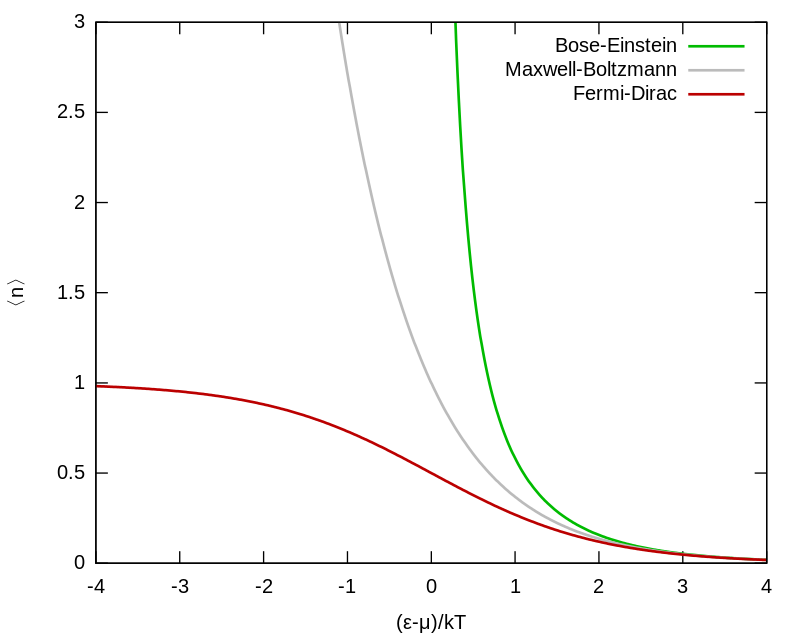
\includegraphics[width=0.5\textwidth]{image.png}
\caption{\label{fig:2}\small \emph{All three distributions}}
\end{figure}
\newpage
\section{Gases}
\subsection{Ideal mono-atomic gas}
\begin{itemize}
    \item We would like to be able to calculate the entropy of a mono-atomic gas. To do this we start with a particle in a box of volume $V=L^3$. Analyzing this system with the Schr\"odinger equation we find that the energy of the particle is given by $\epsilon =\frac{\hbar^2\pi^2}{2mL^2}(n_x^2+n_2^2+n_z^2) $. If we then look at the partition function for this single particle we can make the approximation that these energy levels are very close together for typical values of $m$ and $L$:
\begin{bux}
    \begin{split}
         Z = \sum_{n_x}\sum_{n_y}&\sum_{n_z}e^{-\frac{\epsilon}{kT}} \approx \int_{0}^{\infty}\int_{0}^{\infty}\int_{0}^{\infty}e^{-\frac{\epsilon}{kT}}dn_xdn_ydn_z\\
& \implies Z_0 = V\left(\frac{2\pi mkT}{h^2}\right)^{3/2}
    \end{split} 
\end{bux}
For simplicity we usually call $\frac{N}{V} =\frac{1}{V}= n_c$ the number of particles per unit volume, and $\left(\frac{2\pi mkT}{h^2}\right)^{3/2} = n_Q$ the quantum concentration as it can be shown this is equivalent to one atom in a cube with side length of the de Broglie wavelength $\lambda=\frac{h}{p}$ and $\epsilon=\frac{3}{2}kT$.  This all means $Z_0= \frac{n_Q}{n_c}$.   

\item If we then have $N$ particles in our box we know the sum over all occupation states, given for Maxwell Boltzmann by \ref{eqn:3.21}. This tells us: 
\begin{bux}
    \begin{split}
         N = \sum_i&e^{\frac{\mu-\epsilon_i}{kT}} =  e^{\frac{\mu}{kT}}Z_0\sum_ie^{\frac{-\epsilon_i}{kT}} = e^{\frac{\mu}{kT}}Z_0\\
&\implies   \mu = kT\ln(\frac{n_c}{n_q})
    \end{split}
\end{bux}
As $\frac{N}{V} = n_c$.  We can then use this to solve for the Helmholtz free energy as $\mu = \left(\frac{\partial F}{\partial N}\right)_{\small T,V}$, so:
\begin{bux}
    \begin{split}
        F = \int_0^NkT\ln(\frac{n_c}{n_q})dN = kTN\left(\ln \frac{n_c}{n_q} -1\right)
    \end{split}
\end{bux}
We could also stick to sums and say $F = kT\sum_{n=1}^N\ln(N)-kTN\ln(n_QV)$. Then using the approximation $\sum_{n=1}^N\ln(N) \approx \int_0^N\ln(N)dN  = N\ln(N)-N \approx \ln(N!) $. Which means that:
\begin{flalign}
F  = - kT\ln\left[\frac{Z_0^N}{N!}\right] \implies Z = \frac{Z_0^N}{N!}
\end{flalign}
Which is expected. 

\end{itemize}












\end{document}